
\documentclass[11pt,journal]{IEEEtran}


\usepackage{cite}
\usepackage[pdftex]{graphicx}
\usepackage[tight,footnotesize]{subfigure}
\usepackage{fixltx2e}
\usepackage{float}
\usepackage{hyperref}
\usepackage{slashbox}
\usepackage[english]{babel}

% correct bad hyphenation here
\hyphenation{op-tical net-works semi-conduc-tor}


\begin{document}

\title{CSE 471 Project Write-up \\ Team 2}

\author{\IEEEauthorblockN{David Ganey, Kerry Martin, Evan Stoll, Michael Theut, and Ben Roos\\}
\IEEEauthorblockA{School of Computing, Informatics and Decision Systems Engineering\\
Arizona State University\\
CSE 471\\}
}

% make the title area
\maketitle

\renewcommand{\abstractname}{Executive Summary}
\begin{abstract}
The CEO of CactusCard has commissioned a team to solve several problems facing the up-and-coming financial company. The company is in the process of releasing a new card, called the CactusCardPlus. In order for this new product to be a success, the CEO recognizes that CactusCard Credit must accomplish three distinct goals. First, the company needs to successfully market the new card, through both traditional strategies and in particular to users of social media. In addition to a powerful marketing campaign, the company must ensure it makes good decisions about which applicants are deserving of a line of credit. Failing to do this would put the company at a disadvantage, relative to the numerous credit agencies who do use data to make credit decisions. Finally, the success of the product hinges on its ability to protect users (and the company) from credit card fraud. As such, the team must be prepared to counter fraudulent users through a variety of strategies.
\par
These tasks were undertaken by a team of computer science students with knowledge of artificial intelligence. Using search algorithms, the team maximized the marketing potential of the card. Using machine learning techniques, the team utilized data to accurately predict which applicants will best utilize their line of credit. Using game theory, the team developed successful counter-fraud strategies which can be used to protect the company. 
\par
First, the team needed to market the card effectively. Using 10 cards with no sign up fee and 0\% interest for one year, CactusCard Credit strategically generated interest in the product. Using search techniques described below in Section \ref{part1}, the team devised both simple and complex algorithms which find the optimum individuals to receive these free cards in order to maximize the number of their friends who sign up for the product. The team developed a depth-first search solution as well as a heuristic (A*) search solution. Memory restrictions meant that the A* search did not run efficiently and thus presents a conundrum. With more available computational resources, A* would more efficiently find an optimal solution, but given the resources available, DFS will find a workable solution in less time.
\par
After devising a successful marketing strategy, the team turned its focus to the determination of credit worthiness. As seen below in Section \ref{part2}, the team used a well-known machine learning library called Weka to run various machine learning algorithms on the data set provided. This data set, which contained 15 anonymized credit attributes plus whether or not that individual was given a card, was used to train learning machines which were then evaluated on their ability to accurately predict the issuance decision. After running several tests, the team concluded that a Support Vector Machine run using Weka's implementation of the Sequential Minimal Optimization algorithm was the most effective, both in terms of percentage of individuals correctly classified and in terms of runtime. This SVM algorithm will be an effective choice for CactusCard Credit in the future, and the team has confidence in the correctness of Weka's implementation.

\par
Finally, the team evaluated strategies to defend the company against malicious and fraudulent attacks. The team concluded that, unlike a typical game-theory situation, both players do not have the something to gain. The best case scenario for the defender is simply to minimize losses. Knowing this, the team determined that the defender’s goal in this game should to try to spend the least amount of money while attempting to make the game end as quickly as possible. The best way to do this is to ensure that the attacker never makes any money over a repeated game, but we don’t waste money defending extra vectors. This logic dominates our thinking for the MUCM model. We were successful at employing this model in several different scenarios which are detailed in Section \ref{part3}.
\par
With a Deterministic Adversary with Memory (DAM) model, the team evaluated situations where the attacker and defender each pick a single attack vector per turn. Both players store M memories of previous choices of attach vectors. Through solutions explored in detail below, the team determined that the best choice for CactusCard Credit is to pick the defense vector from memory. Ultimately, however, the team recommends not allocating defense resources to a DAM model strategy.
\par
A third model, based on the DAM model, is an improvement over the DAM model by allowing the attacker and defender to pick more than one vector, but never more than the allowed memory, per round similar to how MUCM picks strategies. It also makes the cost per attack a non-static parameter.
\par
Ultimately, the findings expressed in the study below will benefit CactusCard Credit in multiple ways. By implementing the proposals below, the team believes it will be able to increase the marketing effectiveness of the company, ensure the accuracy of credit issuance decisions, and counter potential fraudulent threats. These decisions will be critical to the future success of the company.
\end{abstract}
\newpage

\IEEEpeerreviewmaketitle

\section{Part 1} \label{part1}
The first part of the project requires the development of search programs to optimize marketing within a social network. Using a dataset given to the study team by the marketing department, the team must propose multiple search-based solutions and document their success. This section will formulate this problem and describe the steps taken to solve it.

\subsection{Problem Importance}
For a new product such as the CactusCard Plus, the initial marketing wave may determine whether the product success or fails. This importance of this period, as the product begins to build a user base, cannot be overstated. Even more critical is the fact that the marketing department wishes to give out some of the cards for free. It is critical that the team choose the right users to receive these free cards such that the impact of those cards in their friend network is the largest.

\subsection{Problem Formulation}
The goal of the problem is to find the optimal distribution of 10 cards such that the most individuals adopt the card. This means that in traversing the relationships established in the input file, the program should find points to deliver free cards where the cards have the desired effect (increasing exposure to the card) without having an undesired side effect (namely, giving too many free cards to a small group and failing to expose other clusters entirely). By using a na{\"i}ve solution combined with a heuristic-based solution, the team can guarantee it will provide an optimal answer. The problem was formalized as a maximization problem, rather than as a minimization problem, because the goal was the maximize the expected number of adopters based on each individual's probability of adoption. Accordingly, the problem formalization includes a reward function rather than a path cost and step cost. The problem was formalized as follows. Goal: Distribute 10 cards. Initial state: No individual has been offered a free card, and no individuals have been exposed to the card. Transition function: Offer a free card to an individual who has not yet been exposed to the card or accepted a free card already. States: The set of possible distributions of free credit cards such that every card that is offered is accepted. Reward: The total number of expected adopters at a given step.

\subsection{Solution Proposals}
The social network information given by the marketing department takes the form of a graph of friends. Each row of the dataset indicates a bidirectional relationship between two individuals. The goal is to give out one free card per day for 10 days. After giving a card, we can track the friends of the individual who received the card (``exposed" individuals) and determine the probability that they sign up for CactusCard Plus. If we sum the individual probabilities of adoption, we have the total number of expected adopters. Strategically distributing these cards in the friend network will maximize the number of sign ups.
\par
Two solutions are proposed. The first solution to this search problem uses a simple depth-first search, while the second solution uses A* search with an admissible heuristic function.

\subsection{Test Plan}
To test these solutions, we will run the corresponding programs until either a goal node is found, at which point the program would end, or running the program becomes computationally infeasible; this could occur because of time restrictions or because of insufficient memory for the program to continue running. We will compare the reward of the goal node found by DFS with the result of the A* search, whether that is an actual goal node, or a node at a higher depth. We will also compare the efficiency of these two programs in terms of exploration of the search tree.

\subsection{Solution 1}
DFS is not an optimal algorithm, so it is highly unlikely that this technique will yield the optimal solution. However, because DFS is complete, it is guaranteed to find at least one goal state, meaning that it will find one sequence of 10 individuals such that all 10 will accept a free card. In this implementation, written in Java, each node in the search tree keeps track of the individuals who have been given cards, the individuals who have been exposed to cards, and the total number of expected adopters at that node. The total number of expected adopters is calculated by summing each individual's probability of adoption and adding the individuals who have already been given cards. At each step of the search, the function will generate all possible successor based on which individuals have not yet been exposed to the card. As each node is generated, it is added to a LIFO stack that keeps tracks the nodes that have not yet been visited. This stack is called the frontier. At each step, a new node is removed from the stack and its successors are subsequently generated and added to the top of the queue. Once the tree reaches a depth of 10 (where the initial state is at depth 0), we know that 10 individuals have accepted the free card, which is a goal node. At this point, the function returns the goal node, and the subsequent solution is printed to the console. The code used for the DFS solution, and the output of that solution, can be found in the Appendix.

Depth-first search has a general-case time complexity of $O(b^d=m)$, where b is the branching factor and m is the maximum depth of the tree. Because the goal state is always at depth 10, it is not possible for the depth of the tree to ever exceed 10; thus, m = 10. The worst case for the branching factor will be the total number of individuals, n. Thus, the worst cast time complexity will be $O(n^{10})$. The general-case space complexity of DFS is $O(bm)$. For the reasons stated previously, the space complexity of this solution will be $O(10n)$.

\subsection{Solution 2}
The A* search solution proposed here functions similarly to the above DFS solution in several ways. At each step, this search technique is nearly identical; a new node is removed from the queue and its successor nodes are subsequently generated and added to the queue. A key difference is that the queue used in A* search is a priority queue based on the reward function, where nodes with higher rewards are closer to the top of the queue, while nodes with lower rewards are closer to the bottom of the queue. In this case, the reward function also includes a heuristic. While the DFS solution used a reward function f(n) = g(n), where g(n) was the total number of expected adopters, the A* solution uses f(n) = g(n) + h(n), where h(n) is a heuristic function to estimate the reward from the current state to the goal state. Because this was a maximization problem, and admissible heuristic would be an estimate that never underestimated the reward from the current state to the goal (this is in contrast to a minimization problem, in which an admissible heuristic would never overestimate the cost).

The heuristic function used for the solution was the total number of individuals who had not yet been exposed to the card. We know that this will never underestimate the total number of expected adopters from the current state to the goal because there's only one scenario in which the total number of expected adopters would ever equal the total number of individuals who hadn't been exposed. In this scenario, you would need to give a free card to every individual who had not yet been exposed. For this to occur, none of the individuals who had not been exposed could be friends, because a connection between two of these individuals would mean that giving a card to one of them would expose the other to the card, and you could no longer give a card to the exposed individual. It would also mean that every single individual would have either been exposed to the card or given the card. From any given state, it is not possible to increase the expected number of adopters any better than by giving a free card to every remaining non-exposed individual. In any other scenario, the total number of expected adopters would be lower than the number of non-exposed individuals remaining. For that reason, we know that this heuristic will never underestimate the actual reward.

In this case, because the problem was formalized as a maximization problem, the heuristic would be consistent if it was \textit{at least} equal to the step reward to an successor node, plus the estimated reward from that successor to the goal. We know that this heuristic is consistent based on the following reasoning. From any state, the step reward to a successor will be 1 + sum(probability of adoption of individuals exposed at this step). The estimated reward from that successor to the goal will be the number of people who have not yet been exposed. The only way that this calculation can yield a result as high as the heuristic estimate from the predecessor state would be if no one was exposed at the successor state. The result would be that the step reward plus the estimated reward to the goal would be equal to the estimated reward to goal from the predecessor. In any other case, if some individuals were exposed at the successor state, then the estimated reward to goal would be lower, and the added reward from the probability of exposed individuals adopting the card would always be lower than the decrease in the estimated reward (because the probability of the exposed individuals adopting the card will always be less than 1). Based on this reasoning, we know that the heuristic is also consistent.

Because a heuristic function was used in calculating the expected reward for each state, the next node to be expanded was not determined on a LIFO basis (as it was in the DFS solution), but was determined based on which state was expected to lead to the path with the highest reward. Furthermore, because the heuristic used in this problem formulation was both consistent and admissible, we know that A* will perform optimally, meaning that the solution found yields the optimal reward, i.e. the maximum number of expected adopters. In order to prevent the algorithm from using an estimated reward on the goal node, and instead use the actual reward, the heuristic reward calculation included a condition to check whether the new state was a goal. If it is a goal, the heuristic reward is set to 0, so the new state will be added to the priority queue based on the actual, not estimated, reward. The code used for the A* solution, and the output of that solution, can be found in the Appendix.

\subsection{Results}
The depth-first technique described above was significantly faster to find a solution than A* search. To a certain extent, this result was anticipated, given the previously-stated inevitable result that a goal would be found at depth 10. Thus, for the DFS technique to find a solution, it only needed to touch 10 nodes. To find the first possible goal, the DFS algorithm took less than 1 second. However, as previously mentioned, depth-first search is not an optimal search technique, making it highly unlikely that the first goal node found was an optimal goal. To determine if there was goal node with a higher reward, we ran a modified version of DFS that continued searching the tree indefinitely for goal nodes, and at every goal, it determined the optimal reward at that point. Although this modified version of DFS never terminated due to computational restrictions of both time and memory, it was clear that the first solution found was not optimal, given that goal nodes with higher rewards were found. This result is shown in Figure 1. While the first goal found by DFS had a reward of 94.847, the highest reward found before terminating was 122.628, showing that a higher reward was possible. 

Due to memory restrictions, the A* search algorithm always terminated before finding a goal node. However, from inspecting the output generated by the function, it was clear that the A* technique was performing optimally prior to its termination. Because A* prioritizes nodes with higher expected reward, and because the expected reward in this problem formulation was based on the number of non-exposed individuals, the algorithm inherently prioritized paths of individuals with fewer friends, because those paths maximized the number of non-exposed individuals. Of course, in the long-term, as those paths are be expanded further, they will be pushed lower in the priority queue because other paths will emerge with a higher expected reward. In this way, an optimal goal will eventually be found. However, because of the prioritization of low-exposure individuals, the A* technique was not able to generate a high-reward path for any depth. In our tests, the deepest path generated by the algorithm reached depth 7, but the reward was significantly lower than the goal found by DFS, and was likely the lowest, or one of the lowest, possible rewards at that depth. The actual reward for that path was only 4.222. This result, however, actually tells us that the A* algorithm was performing as expected. The fact that the path found at depth 7 had extremely low actual reward indicates that the estimated reward, using the heuristic of non-exposed individuals, was very high, showing that the algorithm was prioritizing paths with high estimated reward. Given additional time, we can extrapolate these results to predict that the A* algorithm would continue to pursue those high-reward paths until depth 10, at which point those paths would be sent to a much lower position in the priority queue because the actual reward was so low, and the algorithm would continue until ultimately finding an optimal path. The results are shown below.

\begin{figure}[H]
\centering
    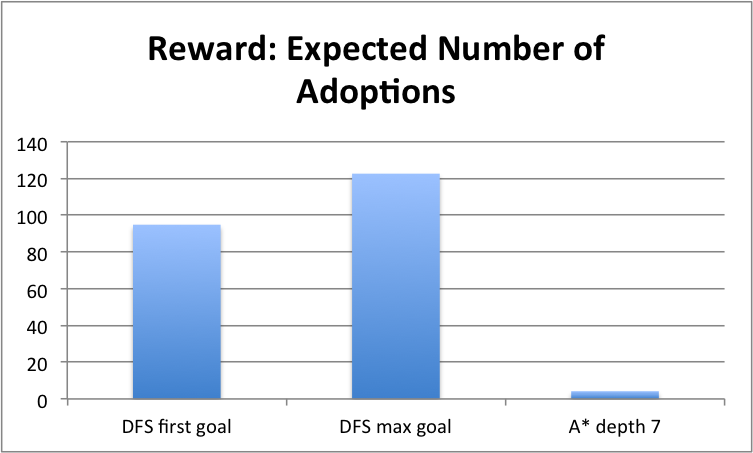
\includegraphics[width=3in]{images/part-1-results}
\caption{Reward for DFS and A* search}
\label{part-1-results}
\end{figure}

Although these results may appear to indicate that DFS performed more optimally than A* search, it actually simply demonstrates that relative inefficiency of A* for this particular problem, and the memory constraints of this implementation. While A* would be faster than DFS at finding an optimal solution (since DFS would have to explore the entire tree), DFS is more efficient at finding a single solution, given that all goal nodes are at depth 10. While DFS can simply explore one subtree to that depth, A* spends more time searching shallower subtrees and jumping between subtrees of different depths to find that path with that highest estimated reward. This result is shown in the table below, demonstrating that even when A* search was depth-limited, it still took much longer to find a path than DFS.

\begin{table}[H]
\centering
{\renewcommand{\arraystretch}{1.2}%
\begin{tabular}{ | p{2.5cm} | l | l | l | }
\hline
Time for DFS to find goal         & 1 second           \\ \hline
Time for A* to reach depth 7    & 9 seconds             \\ \hline
\end{tabular}} \quad
\caption{A table showing the computation times for DFS and A* search}
\end{table}

In this case, because A* only reached depth 7, the path with the highest \textit{estimated} reward was, for reasons stated previously, a path with low \textit{actual} reward.

\section{Part 2} \label{part2}
Part 2 of the project describes another task given by the CEO of the CactusCard Credit Company, wherein a program should be developed to provide ``a \emph{machine learning based approach} to identify individuals who should/should not be given the CactusCardPlus.'' This section will formulate this problem and describe the steps taken to solve it.

\subsection{Problem Importance}
The decision whether or not to grant a line of credit (and, as a corollary, how large that line of credit should be) is one of the most important decisions made by a credit agency. In this age of big data, agencies which fail to accurately utilize existing data to make these decisions are likely to fall behind agencies who are doing so. In this problem, CactusCard Credit is fortunate to have a dataset which tracks many credit attributes for a large number of users.

\subsection{Problem Formulation}
The problem itself is a machine-learning problem, which at its core simply means a program designed to recognize patterns. Machine learning can encompass a wide variety of problems, which can be divided into ``regression'' problems and ``classification'' problems. In this case, the consumer research division has given the team a dataset which contains information about customers \emph{for whom the decision to award or not to award the CactusCard has already been made}. This is important information -- because customers can either be given the card or not (a binary \emph{classification}), this falls under the realm of classification machine learning problems. Additionally, the fact that the classification program will be trained with data means this is a \emph{supervised} learning problem.
\par
As a supervised classification machine, the program must be able to read the data set and, with that information, draw conclusions about which credit variables have the largest impact on whether or not the customer was given the card. To be an effective tool for the CactusCard corporation, the dataset supplied by the consumer research division should only include proper decisions -- cases where the card was awarded to the correct individual and denied to individuals who would have abused the line of credit. Otherwise, the machine will learn ``bad habits'' and will draw conclusions from the data which are not useful to the company.
\par
The dataset itself is comprised of 15 credit attributes for the individuals, as well as an indication of whether the individual received a card. The credit attributes are not specified, though the problem specification does include the data types for each attribute. (For example, attribute 1 can be either ``b'' or ``a'', and therefore represents some binary information about the customer such as whether they are male or female). These attributes, therefore, are all weighted equally, which may present a disadvantage. Further discussion of this issue can be found in Section \ref{conclusion}. Additionally, it is important to note that the dataset is approximately balanced --- approximately half of the individuals were granted cards, while half were not. This is helpful in correctly training the classifier.
\par
The goal of this component of the project is to determine an algorithm which will effectively use the dataset to learn how the credit attributes affect the decision to award the card, and from there use that knowledge to predict card decisions within a certain degree of accuracy.

\subsection{Solution Proposals}
Weka, a software tool developed at the University of Waikato, is a software package with implementations of a large number of machine learning algorithms. Weka can be used in multiple ways. One option is to simply use the Weka API to access the algorithms from Java code. This is advantageous when one wishes to write a full machine learning system, or integrate machine learning algorithms with an existing Java system. Another option is to use the Weka Explorer, which is a wrapper around the algorithms. This GUI tool allows the user to load a data set and run the algorithms on it, then view the results in various formats.
\par
It is the latter method which is proposed to solve the task given by the CEO. Using the Weka Explorer, we have a straightforward method for gaining insight into the effect of the 15 credit attributes. We can use the Explorer to test various machine learning algorithms, and based on their success rates, determine which should be used in the future to make the actual issue decision. An additional advantage of using this method is that Weka is tested, proven, open-source code. The GitHub repository has nearly 8,000 commits, and therefore represents much more stable code than the team could have produced in the time allotted to this study \cite{wekagit}. This provides greater value for the company.

\begin{figure}[H]
\centering
    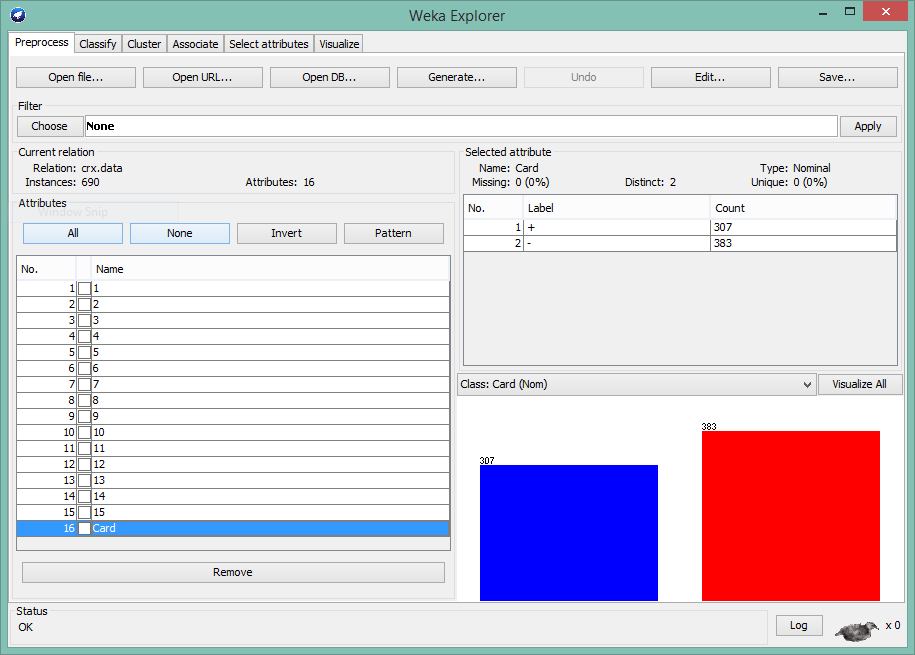
\includegraphics[width=3in]{images/wekaexplorer}
\caption{The Weka Explorer interface}
\label{wekaexplorer}
\end{figure}

\subsection{Test Plan} \label{testplan}
The team will evaluate several popular machine learning algorithms in the Weka Explorer. The success of each algorithm will be determined by a number of factors. The team must consider runtime, as the algorithm cannot take an extreme amount of time to complete or it will be useless. The most important factor, however, is the accuracy of the classification. Using random chance to classify card issuance would theoretically have an accuracy rate of approximately 50\%, so the team must find an algorithm with a higher percentage than that. To ensure CactusCard's continued financial success, the algorithm must predict card issuance correctly at least 80\% of the time. The team proposes this number as it represents a realistic target for algorithms which make mistakes, yet still shows a tremendous potential advantage for CactusCard Credit.

\subsection{Solution 1}
Support Vector Machines (SVM) are, according to Russell and Norvig, ``the most popular approach for `off-she-shelf' supervised learning''' \cite{ai}. SVMs do a good job of classification because they separate groups as much as possible (called a ``maximum margin separator''). Additionally, SVMs can work in multiple dimensions (creating a ``hyperplane'') which will be important with the high number of credit attributes in the data set. Finally, SVMs are considered a non-parametric method, because they store some of the training examples, and yet like parametric models, they often avoid over-fitting the data \cite{ai}.
\par
To use an SVM on the data set provided by the CEO, Weka supports the addition of a library called libsvm. This Java library contains an implementation of the SVM algorithm (called SMO, for sequential minimal optimization) which hooks into the Weka Explorer interface. The team will set the Explorer to use varying numbers of crossfold validation passes, in order to evaluate the classifier. This will split the dataset, train the SVM with a subset of the dataset, and then evaluate the SVM's effectiveness at predicting the card issuance decision by comparing the SVM's predictions to the actual data. The results from running the libsvm algorithm on the dataset are shown in the table below:

\begin{table}[H]
{\renewcommand{\arraystretch}{1.2}%
\begin{tabular}{ | p{2.5cm} | l | l | l | }
\hline
Crossfold validations         & 5             & 10            & 15            \\ \hline
Time taken to build model (s) & .15           & .21           & .16           \\ \hline
Correctly classified (\%)     & 587 (85.07\%) & 586 (84.93\%) & 585 (84.78\%) \\ \hline
Incorrectly classified (\%)   & 103 (14.93\%) & 104 (15.07\%) & 105 (15.22\%) \\ \hline
\end{tabular}} \quad
\caption{A table showing the results of the libsvm applied to the data set}
\end{table}

As we can see from the table, no significant difference appears to exist when adjusting the number of crossfold validation passes. All of the attempts fall well within the expected runtime, and predict with approximately 84\% accuracy whether someone was or was not given a CactusCard. This is well within the criteria established above in Section \ref{testplan}, and thus is a valid contender for the chosen algorithm.

\subsection{Solution 2}
Another type of machine learning algorithm is called a Multilayer Perceptron (MLP). This is a type of neural network, which maps from inputs (in this case, the credit attributes) to outputs (whether someone was given a card). The MLP is suitable for this task because it uses \emph{backpropagation}, which is a supervised learning technique. The network is initialized with random initial weights, then backpropagation algorithm minimizes the error function using the method of gradient descent, which in turn recursively updates the initial weights. By using backpropagation, MLPs are able to handle hidden values which are present in this dataset. Given that MLPs handle such hidden values whereas SVMs do not, we intuitively expect that MLPs may better classify the data.
\par
The Multilayer Perceptron is significantly more complex than the SVM, but conveniently Weka does include an implementation in the Explorer. Using the same technique as above, the team will evaluate this algorithm with various levels of crossfold validation to determine the optimal setting. The results are seen below:

\begin{table}[H]
{\renewcommand{\arraystretch}{1.2}%
	\begin{tabular}{ | p{2.5cm} | l | l | l | }
\hline
Crossfold validations         & 5             & 10            & 15            \\ \hline
Time taken to build model (s) & 8.46          & 8.47          & 8.51          \\ \hline
Correctly classified (\%)     & 584 (84.64\%) & 572 (82.90\%) & 572 (82.90\%) \\ \hline
Incorrectly classified (\%)   & 106 (15.36\%) & 118 (17.10\%) &           118 (17.10\%)  \\ \hline
\end{tabular}
} \quad
\caption{A table showing the results of the Multilayer Perceptron applied to the data set}
\label{fig:mlp}
\end{table}

Once again, it is clear that adjusting the number of crossfold validations has little to no effect on the accuracy of the classifier. As a result, the recommendation of the team is to use 5 validations on data sets of this size, so the algorithm does not take too long to run. While the time taken to build the data model was always nearly the same, the total runtime for all passes of the validation increased dramatically with larger numbers of cross fold validations. Since they appear to have no impact on the effectiveness of the algorithm, there is no need for the program to take that additional time. It is likely that on future datasets with larger numbers of individuals, the runtime would increase further still, reinforcing the decision that 5 crossfold validations is the correct choice.
\par
Although no difference between the columns in Table \ref{fig:mlp} is visible, we can see immediately that the Multilayer Perceptron is a reasonable choice for the CactusCard company. In all cases, the success of the classifier was above the criteria set above in Section \ref{testplan}. The MLP algorithm averaged approximately 83\% correctness, which is significantly higher than random chance. This algorithm would be a good choice for future data sets, where it could use the information it learned from this training set to choose who receives a card.

\subsection{Conclusion}
In summary, both the vector-based classifier and the neural network succeeded at predicting the credit issuance decision with at least 80\% accuracy. Both algorithms are therefore suitable for the company and can be used to make decisions regarding new clients. However, the SVM's performance can be considered better in the context of our evaluation plan, as the time taken to build the model is a fraction of the time taken by the multilayer perceptron. As a result, the team recommends the sequential minimal optimization implementation of the support vector machine for CactusCard Credit.

\section{Part 3} \label{part3}
The third part of the CactusCard project asks us to implement and test two models used to simulate malicious attacks on the card company so that they can better understand how to defend against credit card attacks (fraud, phishing, theft, etc.).

\subsection{Problem Importance}
For a credit card company, security is a top priority. When handling such sensitive data, a security breach can have massive consequences. It makes sense for CactusCard to want to try its best to understand how these attacks work and what methods are best to defend against them. Card companies that have a reputation of not being secure are unlikely to succeed in the business for long. To guarantee the long-term success of CactusCard Credit, robust defense strategies must be developed. 

\subsection{Problem Formulation (DAM model)}
The problem here is a game theory problem wherein an analysis must be performed on the performance of two proposed models for defending against attacks. The game theory models here simulate an attacker and a defender trying to maximize their score by increasing the payoff they receive for either successfully defending or attacking. The attacker and defender both utilize a list of attack vectors that determine the outcome of the game. Both players have to pay a \$100 cost for each attack vector they utilize, but winning the game results in a \$10,000 payoff. For both models their will be 100 possible attack vectors available to the attacker and defender.
\par
One of the proposed models is the Deterministic Adversary with Memory (DAM) model. In this model, both attacker and defender will pick a single attack vector per turn. In a given turn, the defender is considered the winner if it picks the same vector that the attacker picks in that turn, otherwise the attacker wins. Both players will have memory that is used to store the last five attack vectors used by the attacker. We will use M to represent the size of the memory for the attacker and defender. Note that both attacker and defender memory is independent from each other. For the first M turns the attacker and defender will pick an attack vector from the list of vectors uniformly at random, each completely independent of its opponent. After the initial moves each player will choose a vector either from memory or a vector that is not in memory. The probability that a player will choose its vector from memory is determined by a parameter S. S ranges from 0.0 to 1.0, a player will have a 100\% chance to pick from memory with an S = 1.0.

\subsection{Solution Proposals (DAM model)}
For the DAM model CactusCard asks us to find a strategy for the defender that performs better than the attacker in the DAM model. Given that the number of attack vectors is 100 and the number of vectors stored in memory at any point is 5, it makes sense for the defender to try to maximize the number of times both defender and attacker pick their vector from memory. Even if the attacker is unlikely to pick from memory (low S value), it should be more beneficial to always pick from memory since the chance that both the attacker and defender will pick the same not-in-memory vector is very small (1/95). When both attacker and defender pick from memory, the probability for the defender to successfully defend jumps to (1/5). It seems that the best strategy the defender can use is to always pick a vector from memory. 

\subsection{Test Plan (DAM model)}
To test the DAM model alternate strategy, the base DAM model defender strategy will be compared to the alternative defender strategy that we proposed. The base DAM model will be implemented using Java. Testing the alternate strategy for the defender will be simple, we can just leave the S parameter for the defender as 1.0 so that the defender always picks its vector from memory. Using the implementation a series of test will be ran analyzing the average payoff for each player for the different S parameters. The same will be done for the alternative strategy. The two strategies will be compared after the average payoff for the players is gathered.

\subsection{Solution 1 (DAM model)}
Overall the defender performs very poorly in the base DAM model. In the best case scenario, where both defender and attacker have a 100\% chance to pick their vector from memory the defender still only blocks roughly 20\% of the attacks. We took the average number of attacks successfully defended of 20 simulations and compiled them into the table below:


\begin{table}[H]
{\renewcommand{\arraystretch}{1.2}%
\begin{tabular}{ | p{3.2cm} | l | l | l | l | l |}
\hline
\backslashbox{Defense S}{Attack S} 	& 0.0	& 0.25	& 0.5	& 0.75	& 1.0            \\ \hline
0.0  & 5.4 	& 4.3	& 2.6	& 1.4	& 0.2   \\ \hline
0.25 & 4.3	& 8.8   & 12.8	& 17.9	& 25.2   \\ \hline
0.5  & 2.3	& 14.5	& 24.4	& 37.3	& 50.4   \\ \hline
0.75 & 1.8	& 17.2	& 35.1	& 57.7	& 74.3	\\ \hline
1.0  & 0.2	& 23.5	& 46.0	& 71.2	& 100.5	\\ \hline
\end{tabular}} \quad
\caption{Average number of attacks successfully defended (out of 500) attacks by varying S parameters}
\end{table}

Since our proposed alternative strategy was for the defender to simply always pick from memory no further testing was needed. This table not only shows the performance of our base model, but also the performance of our proposed alternative strategy for the defender. Although our alternative model no longer requires an S parameter, its performance can be accurately represented by the table when the defenders S parameter equals 1.0.
\par

Based on these results, the team does not recommend using a defender strategy that follows the DAM model. Choosing this strategy is likely to lead to CactusCard Credit failing to block the majority of the attacks, which will negatively affect our client base.

\subsection{MUCM}

\par Whenever this game is played, CactusCard cannot make money. Since CactusCard can only lose money, the goal then is to make sure that the game is played for the shortest amount of time possible. The most cost-effective way to make sure the game is not played very long is to make sure the attacker is not making any money, and then minimizing our cost while still ensuring that the attacker is not making money.

\par So the goal is to defend the number of attacks that will maximize his losses and minimize the money we spend. 

\par The first priority is to ensure the attacker is losing money. This is computed through determining the expected value. Once we get him losing money, we need to find the optimal amount of vectors to defend that will minimize out losses. The following is our findings when the attacker attacks 1, 2, and 10 vectors.\\

\par
Assuming: Attacker V = 1; Catk = 1000\\

\par
Cost Results:\\

\par
Defender: Assuming they only attack one vector, then we're going to average out to about -\$10000 anyway we play, no matter what the other variables are. The best results I found were defending 97 attacks. That way, the attacker will average out at -\$797.98 and the defender will average out at -\$9902.02.\newline
 

\par
Payoff (97.98\% chance of successful defense):
\par
Successful attack:
Attacker: 9000;
Defender: -19700
\par
Successful defense:
Attacker: -1000;
Defender: -9700\newline

\par
Assuming: Attacker V = 2; Catk = 500\\

\par
Cost Results:\\

\par
Defender: The attacker's next best move is to attack 2 vectors. This time, the most cost effective way to ensure that he doesn't average out to make any money is to defend 68 vectors. This averages out to the defender losing \$41.43 and the attacker losing \$41.43 and the defender losing \$7758.77\newline

\par
Payoff (90.41\% chance of successful defense): 
\par
Successful attack:
Attacker: 9000;
Defender: -16800
\par
Successful defense:
Attacker: -1000;
Defender: -6800\newline


\par
Assuming: Attacker V = 10; Catk = 300\\

\par
Cost Results:\\

\par
Defender: This time the attacker attacks 10 vectors. The best response when the defender is paying \$300 per attack is to defend 22 vectors. This still gives a likelihood of defense at 92.96\% and averages out the defender to lose \$2192.31 per round the defender to lose \$2907.69\newline

\par
Payoff (92.96\% chance of successful defense): 
\par
Successful attack:
Attacker: 7000;
Defender: -12200
\par
Successful defense:
Attacker: -3000;
Defender: -2200\newline

\par
One of the most equal options is when the attacker’s cost is \$500, and attacks 10 vectors. If we defend 15 vectors, this has an 82.28\% chance of a successful defense.

\par
This will average out to an expected value of -\$3227.76 for the attacker and -\$3272.24 for the defender.

\par
Overall, the reasonable investment for the company entirely depends on the amount of attack vectors that the attacker decides to play. The fewer he plays, the more expensive it is for the company.

\subsection{New Model}
A new implementation, combining aspects of the MUCM and DAM consists of setting up the model similar to the DAM. Instead of a static cost per attack vector, use parameters for cost $C_{atk}{*}$ and $C_{def}{*}$ for the attacker and CactusCard, respectively.
\par
A second change is to select $X_{atk}$ vectors, where $X_{atk} \leq M_{atk}$ and chosen randomly. The probability of selecting one of the previous $M_{atk}$ moves is then given by
\[S_{atk} - \prod_{i=0}^{X_{atk}} \frac{X_{atk}-i}{M_{atk}}\]
The probability of picking a move not in memory is still $1-S_{atk}$ (uniformly at random). The defense is the same as the attack, but replacing $S_{atk}$, $X_{atk}$, $M_{atk}$ with $S_{def}$, $X_{def}$, $M_{def}$
\par
This model is no longer limited in the same way as the DAM because it no longer selects only one attack vector in each round $N$. Instead, it selects a random number of attack vectors from vectors in its memory and from vectors not in its memory. This is a more complex model that better encapsulates the idea that attackers are not restricted to only one attack vector. It still relies on memory $M_{atk}$ and $M_{def}$, and it gives greater freedom to choose parameters $C_{atk}*$ and $C_{def}*$ which can better represent actual costs, rather than using a static value.
\par
A successful attack for the attacker has payoff \[S.P_{atk} = B_{atk} -\sum_{v \in V_{atk}} C_{atk}*\] 
\par
For the defense, a successful attack has payoff \[S.P_{def} = -B_{atk} -\sum_{v \in V_{def}} C_{def}*\]
\par
Unsuccessful attacks have payoffs \[U.P_{atk} = -\sum_{v \in V_{atk}} C_{atk}*\] \[U.P_{def} = -\sum_{v \in V_{def}} C_{def}*\] for the attacker and defender, respectively. In these payoffs, $V_{atk}$ and $V_{def}$ are each of the vectors used by the attacker and defender.
\par
The payoff matrix for this new model for a successful attack or successful defense relies on whether $V_{atk} \cap V_{def} = \emptyset$ for Case 1, or $V_{atk} \cap V_{def} \neq \emptyset$ for Case 2. Using the definition of independence of sets in a probability space $P(A \cap B) = P(A)\cdot P(B)$
\[P( V_{atk} \cap V_{def}) =\]
\[ V^2 ( 1 - \prod_{i=0}^{X_{atk}} \frac{X_{atk}-i}{M_{atk}}) ( 1 - \prod_{j=0}^{X_{def}} \frac{X_{def}-j}{M_{def}}) \]

Combining these probabilities and the payoffs gives the payoff matrix for this new model.
 \begin{table}[H]
{\renewcommand{\arraystretch}{1.2}%
\begin{tabular}{ |l |l | l | }
\hline
Payoffs & Case 1  & Case 2  \\ \hline
Attacker & $P(V_{atk}\cap V_{def})(S.P_{atk})$ & $(1-P(V_{atk}\cap V_{def}))(U.P_{atk})$    \\ \hline
 Defender  & $P(V_{atk}\cap V_{def})(S.P_{def})$ & $(1-P(V_{atk}\cap V_{def}))(U.P_{def})$  \\ \hline

\end{tabular}} \quad
\caption{A table showing the payoff matrix using the combined model of MUCM and DAM} 
\end{table}


\section{Conclusion} \label{conclusion}
The conclusion goes here.
Discuss issues with part 2 dataset -- all attributes weighted equally


% use section* for acknowledgement
\section*{Appendices}

The source code for this assignment can be found at:
\url{https://github.com/dhganey/471-project}


\section*{Work}
All team members contributed significantly to the project. Ben Roos worked on Part 1. David Ganey and Kerry Martin worked on Part 2. Evan Stoll and Michael Theut worked on Part 3. All team members contributed to the write up and the presentation slides.


\begin{thebibliography}{1}

\bibitem{rojas1996neural}
Rojas, Ra{\'u}l, \emph{Neural networks: A Systematic Introduction}\hskip 1em plus
  0.5em minus 0.4em\relax Springer Science \& Business Media, 1996.

\bibitem{ai}
S. Russell, P. Norvig, \emph{Artificial Intelligence: A Modern Approach}\hskip 1em plus
  0.5em minus 0.4em\relax Prentice Hall, 2009.

\bibitem{wekagit}
\emph{weka mirror with git} \hskip 1em plus
  0.5em minus 0.4em\relax The University of Waikato.

\end{thebibliography}



% that's all folks
\end{document}


